\documentclass{article}
\usepackage[utf8]{inputenc}
\usepackage{amsmath}
\usepackage{algorithm}
\usepackage{algpseudocode}
\usepackage{graphicx}

\usepackage[margin=2.2cm]{geometry}

\title{Theory Assignment-4: ADA Winter-2024}
\author{Vikranth Udandarao (2022570) \and Ansh Varshney (2022083)}

\date{}
\begin{document}

\maketitle


\section{Preprocessing and Assumptions}
    In this problem, we preprocess, assume or have been given the following:

    \begin{enumerate}
        \item The graph $G = (V, E)$ is a directed acyclic graph (DAG) and is given to us in the problem.
        \item Two vertices $s$ and $t$ are specified in the graph.
        \item The graph has $n$ vertices and $m$ edges.
        \item The vertices of the graph are labeled from 0 to n-1.
        \item A vertex v is defined as (s,t) cut if it is present in all the paths that can be possible from s to t. Vertex v cannot be s or t.
        \item Graph has been given to us in the form of an adjacency list, i.e. stores the list of outgoing vertices for each vertex.
        \item In the Sample Test Case, Vertex a is s $(Source)$ and Vertex e is t $(Destination)$.
    \end{enumerate}


\section{Problem Formulation as a Graph Theoretic Problem}
    We know that we must find the vertices in all paths from s to t. This is equivalent to saying that on the removal of any of these vertices, we cannot reach from s to t. So, we formulate the problem as finding all vertices that, when removed, disconnect the path from $s$ to $t$ in a directed acyclic graph (DAG). This can be represented by constructing a graph where vertices are the nodes of the original DAG and edges represent the dependencies between nodes. If we take a theoretical example, nodes represent tasks in a project scheduling scenario, and directed edges represent dependencies between tasks. We can construct the graph from the adjacency list that we assume will be given to us. It has the outgoing vertices for each vertex of the graph.

    \textbf{Example:}
        Consider a graph $G$ with vertices $s, A, B, C,$ and $t$ such that $s \rightarrow A \rightarrow B \rightarrow C \rightarrow t$. Here, vertices $A, B,$ and $C$ are (s, t)-cut vertices as removing any of them disconnects the path from $s$ to $t$.


\section{Algorithm Description}
    We traversed the graph twice for this algorithm, each time using DFS. In the first traversal, we found a topological sorting of all the vertices (using DFS and stack). Since graph G is DAG, it can be linearly ordered topologically, and its topological sort will contain all the vertices. Then, we used a modified DFS based function FindCutNodes to identify which vertices are (s,t) cut.

    \subsection{Topological Sort Description}
    The Topological Sorting has been done in the following way:
        \begin{enumerate}
            \item Initialize an empty stack that will store the topological sorting.
            \item Initialize a visted$_$topo array that has n elements all initialized as 0 initially. This array will have value 0 if a vertex is not visited and 1 if it has been visited.
            \item Perform a DFS traversal starting from vertex $s$.
            \item When visiting a vertex $v$ during DFS, mark it as visited,i.e., visited$_$topo[v]=1.
            \item Now iterate through all its neighboring vertices and call the DFS function recursively for all the vertices $u$ that are not visited, i.e., visited$_$topo[u]=0.
            \item After iterating through all the neighbors of $v$, push $v$ into the stack.
            \item At the end, after all the vertices have been visited, the stack (from top to bottom following LIFO) will contain the topological sorted order of all the vertices. 
        \end{enumerate}

    \subsection{Modified DFS (FindCutNodes) Description}
    The FindCutNodes is as follows:
        \begin{enumerate}
            \item Initialize an empty set or list to store cut vertices. Call it cutnodes.
            \item Initialize an array start with n elements all equal to 0 initially. This array will store 1 if a vertex is visited (basically denotes entry during DFS).
            \item Initialize an array end with n elements all equal to 0 initially. This array will store 1 if a vertex has been visited back, i.e., recursive calls for all the neighbors of this vertex have been made, and we have returned back to this vertex (basically denotes exit during DFS).
            \item Perform DFS traversal in the topologically sorted order,i.e., call the FindCutNodes function for stack elements (in LIFO order) whose start value is 0 and pop the element from stack after the function has been called.
            \item When visiting a vertex $v$ during FindCutNodes function:
            \begin{itemize}
                \item Update start[v]=1.
                \item For each outgoing edge ($v, u$):
                \begin{itemize}
                    \item If $u$ has start[u] equal to 0 (the node has not been visited before) call the function again recursively for this node.
                    \item Else if suppose start[u] is 1 but end[u] is 0, that means that our necessary condition for (s,t) cut vertex has been satisfied. This implies that u is a (s,t) cut vertex. Add it to the cutnodes array.
                \end{itemize}
            \end{itemize}
            \item After this, mark end[v]=1, showing that the traversal for this vertex has been done.
            \item After calling this function for each vertex, the cutnodes array will contain all the nodes that when removed will lead to no path left between s and t in the graph, i.e. all the (s,t) cut vertices.
        \end{enumerate}


\section{Pseudocode}
    \begin{algorithm}
    \caption{findCutNodes}
        \begin{algorithmic}[1]
        
        \Function{TopologicalSort}{$node, st, visited, adj[]$}
            \State $visited[node] \gets 1$ \Comment{Mark the current node as visited}
            \For{$i$ in $adj[node]$} \Comment{Iterate through the adjacent nodes}
                \If{$visited[i] = 0$} \Comment{If the adjacent node is not visited}
                    \State \Call{TopologicalSort}{$i, st, visited, adj[]$} \Comment{Recursively call TopologicalSort}
                \EndIf
            \EndFor
            \State $st.push(node)$ \Comment{Push the current node into the stack}
        \EndFunction
        
        \vspace{0.5cm}
        
        \Function{findCutNodes}{$node, start, end, cut\_nodes, adj[]$}
            \State $start[node] \gets 1$ \Comment{Mark the current node as visited (entry)}
            \For{$i$ in $adj[node]$} \Comment{Iterate through the adjacent nodes}
                \If{$start[i] = 0$} \Comment{If the adjacent node is not visited (entry)}
                    \State \Call{findCutNodes}{$i, start, end, cut\_nodes, adj[]$} \Comment{Recursively call findCutNodes}
                \ElsIf{$start[i] = 1$ and $end[i] = 0$} \Comment{If the adjacent node is visited but not exited}
                    \State $cut\_nodes.push\_back(i)$ \Comment{Add the current node to the cut nodes list}
                \EndIf
            \EndFor
            \State $end[node] \gets 1$ \Comment{Mark the current node as exited}
        \EndFunction
        
        \vspace{0.5cm}
        
        \Function{Main}{}
            \State $visited\_topo \gets \text{vector}(n, 0)$ \Comment{Initialize visited array for topological sort}
            \State $adj[] \gets \text{vector of adjacency lists}$ \Comment{Initialize adjacency lists}
            \State $st \gets \text{empty stack}$ \Comment{Initialize empty stack for topological sort}
            \For{$i$ from $0$ to $n-1$} \Comment{Iterate through all nodes}
                \If{$visited\_topo[i] = 0$} \Comment{If the node is not visited}
                    \State \Call{TopologicalSort}{$i, st, visited\_topo, adj[]$} \Comment{Call TopologicalSort for unvisited nodes}
                \EndIf
            \EndFor
            \State $start \gets \text{vector}(n, 0)$ \Comment{Initialize start array for findCutNodes}
            \State $end \gets \text{vector}(n, 0)$ \Comment{Initialize end array for findCutNodes}
            \State $cut\_nodes \gets \text{empty vector}$ \Comment{Initialize empty vector for cut nodes}
            \While{$st$ is not empty} \Comment{While stack is not empty}
                \State $node \gets st.top()$ \Comment{Get the top node from the stack}
                \State $st.pop()$ \Comment{Remove the top node from the stack}
                \If{$start[node] = 0$} \Comment{If the node is not visited (entry)}
                    \State \Call{findCutNodes}{$node, start, end, cut\_nodes, adj[]$} \Comment{Call findCutNodes for unvisited nodes}
                \EndIf
            \EndWhile
            \State \Return $0$ \Comment{Return success}
        \EndFunction
        
        \end{algorithmic}
    \end{algorithm}


\section{Complexity Analysis and Explanation of Running Time}
    \subsection{Time Complexity}
        The time complexity of the algorithm is $O(n + m)$, where $n$ is the number of vertices and $m$ is the number of edges in the graph. This complexity arises from the following key operations:
        \begin{itemize}
            \item Topological sorting using DFS: This operation traverses each vertex and its outgoing edges once, leading to a time complexity of $O(n + m)$.
            \item DFS traversal in the findCutNodes function: This operation also traverses each vertex and its outgoing edges once, contributing to the overall time complexity of $O(n + m)$.
        \end{itemize}

    \subsection{Space Complexity}
        The space complexity of the algorithm is $O(n)$, primarily due to the following data structures and variables:
        \begin{itemize}
            \item Visited array (visited\_topo): This array tracks visited nodes during topological sorting and DFS traversal, requiring $O(n)$ space.
            \item Start and end arrays in findCutNodes: These arrays store information about node traversal states, requiring $O(n)$ space each.
            \item Stack (st): The stack is used for topological sorting and can store up to $n$ vertices, adding $O(n)$ space complexity.
        \end{itemize}


\section{Necessary and Sufficient Conditions explaining the algorithm}
    Any vertex v that is (s,t)-cut vertex will have all paths from s to t pass through v. So, if suppose v is removed from the graph, then there will be no path to reach from s to t. Hence, we need to find the vertices that, when removed from the graph will make t unreachable from s in the graph.
    \\\\
    We have first ordered the DAG in a topologically sorted order so that we do not randomly iterate through the vertices later, as this might increase the time complexity. Topological sorting ensures that every vertex comes before its successors in the ordering. This is crucial because it helps efficiently identify each vertex's ancestors and descendants.
    \\\\
    Then, for a vertex v to be cut vertex, it should not have a back edge from any of its descendants to any of its ancestors. If this is true, then there should not be any child u of v that has a back edge from u's descendant to v's ancestor. This ensures that removing v would disconnect the path between s and t. If there were a back edge from a descendant of v to an ancestor of v, it would create an alternative path bypassing v. Hence, v wouldn't be a cut vertex. We check these conditions by checking that the vertex's start array value is 1 and the end array value is 0. If this is true, then the vertex will be a cut vertex and we will add it to the cutnodes array.

\section{Proof of Correctness}
    
    \textbf{Proof of Correctness by Induction:}
    
    We will prove the correctness of the algorithm using induction.
        
        \textbf{Base Case (k = 1)}
        
            For a graph with only one vertex, the algorithm correctly identifies that the vertex is not an $(s, t)$-cut vertex because it cannot disconnect any path between $s$ and $t$ (since there is no other vertex to connect to).
        
        \textbf{Inductive Step}
        
            Assume that the algorithm correctly identifies $(s, t)$-cut vertices for a graph with $k$ vertices. We will now prove that it also works for a graph with $k + 1$ vertices.
            
            Let's denote the graph with $k$ vertices as $G_k$ and the graph with $k + 1$ vertices as $G_{k+1}$. Now, we add one more vertex to $G_k$ to form $G_{k+1}$.
            
            \begin{itemize}
                \item \textbf{Case 1:} The new vertex added is not connected to any existing vertex.
                \begin{itemize}
                    \item In this case, the new vertex cannot be an $(s, t)$-cut vertex because it does not lie on any path from $s$ to $t$. The algorithm correctly identifies this and does not include it in the cut nodes list.
                \end{itemize}
                
                \item \textbf{Case 2:} The new vertex is connected to existing vertices in $G_k$.
                \begin{itemize}
                    \item Now, let's consider the scenarios:
                    \begin{itemize}
                        \item If the new vertex is connected to $s$ or $t$:
                        \begin{itemize}
                            \item In this case, the new vertex cannot be an $(s, t)$-cut vertex because removing it does not disconnect any path from $s$ to $t$.
                        \end{itemize}
                        \item If the new vertex is connected to vertices other than $s$ and $t$:
                        \begin{itemize}
                            \item In this case, removing the new vertex may or may not disconnect paths from $s$ to $t$, depending on the structure of the graph. The algorithm correctly identifies this by performing DFS traversal and finding all $(s, t)$-cut vertices.
                        \end{itemize}
                    \end{itemize}
                \end{itemize}
            \end{itemize}
            
            By the induction hypothesis, the algorithm correctly identifies $(s, t)$-cut vertices for $G_k$. And from the above analysis, we see that it also correctly handles the addition of one more vertex to form $G_{k+1}$. Therefore, by induction, the algorithm correctly identifies $(s, t)$-cut vertices for any graph $G$ with $k + 1$ vertices.
            
            This completes the proof of correctness by induction.

    \textbf{Soundness:} 
        The algorithm is sound because it only identifies a vertex as an $(s, t)$-cut vertex if the removal of this vertex increases the number of disconnected components, meaning there is no path from $s$ to $t$ that bypasses this vertex. This is verified by the DFS traversal which ensures that each identified cut vertex is on all paths from $s$ to $t$.
    
    \textbf{Completeness:} 
        The algorithm is complete because it performs a thorough DFS traversal starting from the source $s$, considering all possible paths to the destination $t$. During this traversal, it checks every vertex that could potentially be an $(s, t)$-cut vertex by exploring all outgoing edges. Thus, it guarantees that no potential cut vertex is missed.

    CHECK BELOW FOR SAMPLE TESTCASE

        % \newpage

        \textbf{SAMPLE TESTCASE:}
        
        \begin{figure}
            \centering

            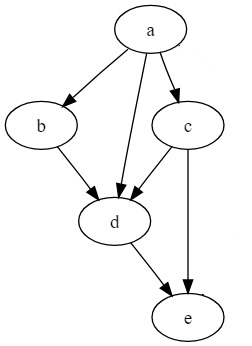
\includegraphics[scale=0.5]{sample-testcase.png}
            \label{fig:enter-label}
        \end{figure}
        
        \textbf{Vertices:}
        \begin{itemize}
            \item a
            \item b
            \item c
            \item d
            \item e
        \end{itemize}
            
        \textbf{Edges:}
        \begin{itemize}
            \item a $\rightarrow$ b
            \item a $\rightarrow$ d
            \item a $\rightarrow$ c
            \item b $\rightarrow$ d
            \item c $\rightarrow$ d
            \item c $\rightarrow$ e
            \item d $\rightarrow$ e
        \end{itemize}
        
        \textbf{Expected Output:}
        
        Cut nodes: d
        
        \textbf{Explanation:}
        
        \begin{itemize}
            \item Vertex $a$ is the source, and vertex $e$ is the destination.
            \item Vertex $d$ is a cut vertex because it is the only point of failure for the paths $a \rightarrow d \rightarrow e$, $b \rightarrow d \rightarrow e$, and $c \rightarrow d \rightarrow e$. Without $d$, there is no path from $a$, $b$, or $c$ to $e$, thus increasing the number of disconnected components from the source to the destination.
            \item Vertices $b$ and $c$ are not cut vertices with respect to the source $a$ and destination $e$. While they do participate in directing the flow of the graph, their removal does not isolate $e$ from $a$ due to alternative paths available ($a \rightarrow d \rightarrow e$ in case of removing $b$, and $a \rightarrow b \rightarrow d \rightarrow e$ in case of removing $c$).
        \end{itemize}
        
        Therefore, the removal of vertex $d$ would prevent access from the source $a$ to the destination $e$, confirming it as the critical cut vertex in the context of directed paths between $a$ and $e$.


\end{document}